\subsection{FHR Benchmark Specifications}

\subsection{FHR Benchmark Results}

\begin{frame}
    \frametitle{FHR Benchmark Phase I-A Results}
    \begin{table}
        \caption{FHR Benchmark Phase I-A (2D assembly steady state model) results 
        \cite{chee_arfcfhr-benchmark_2021}.}
        \only<1>{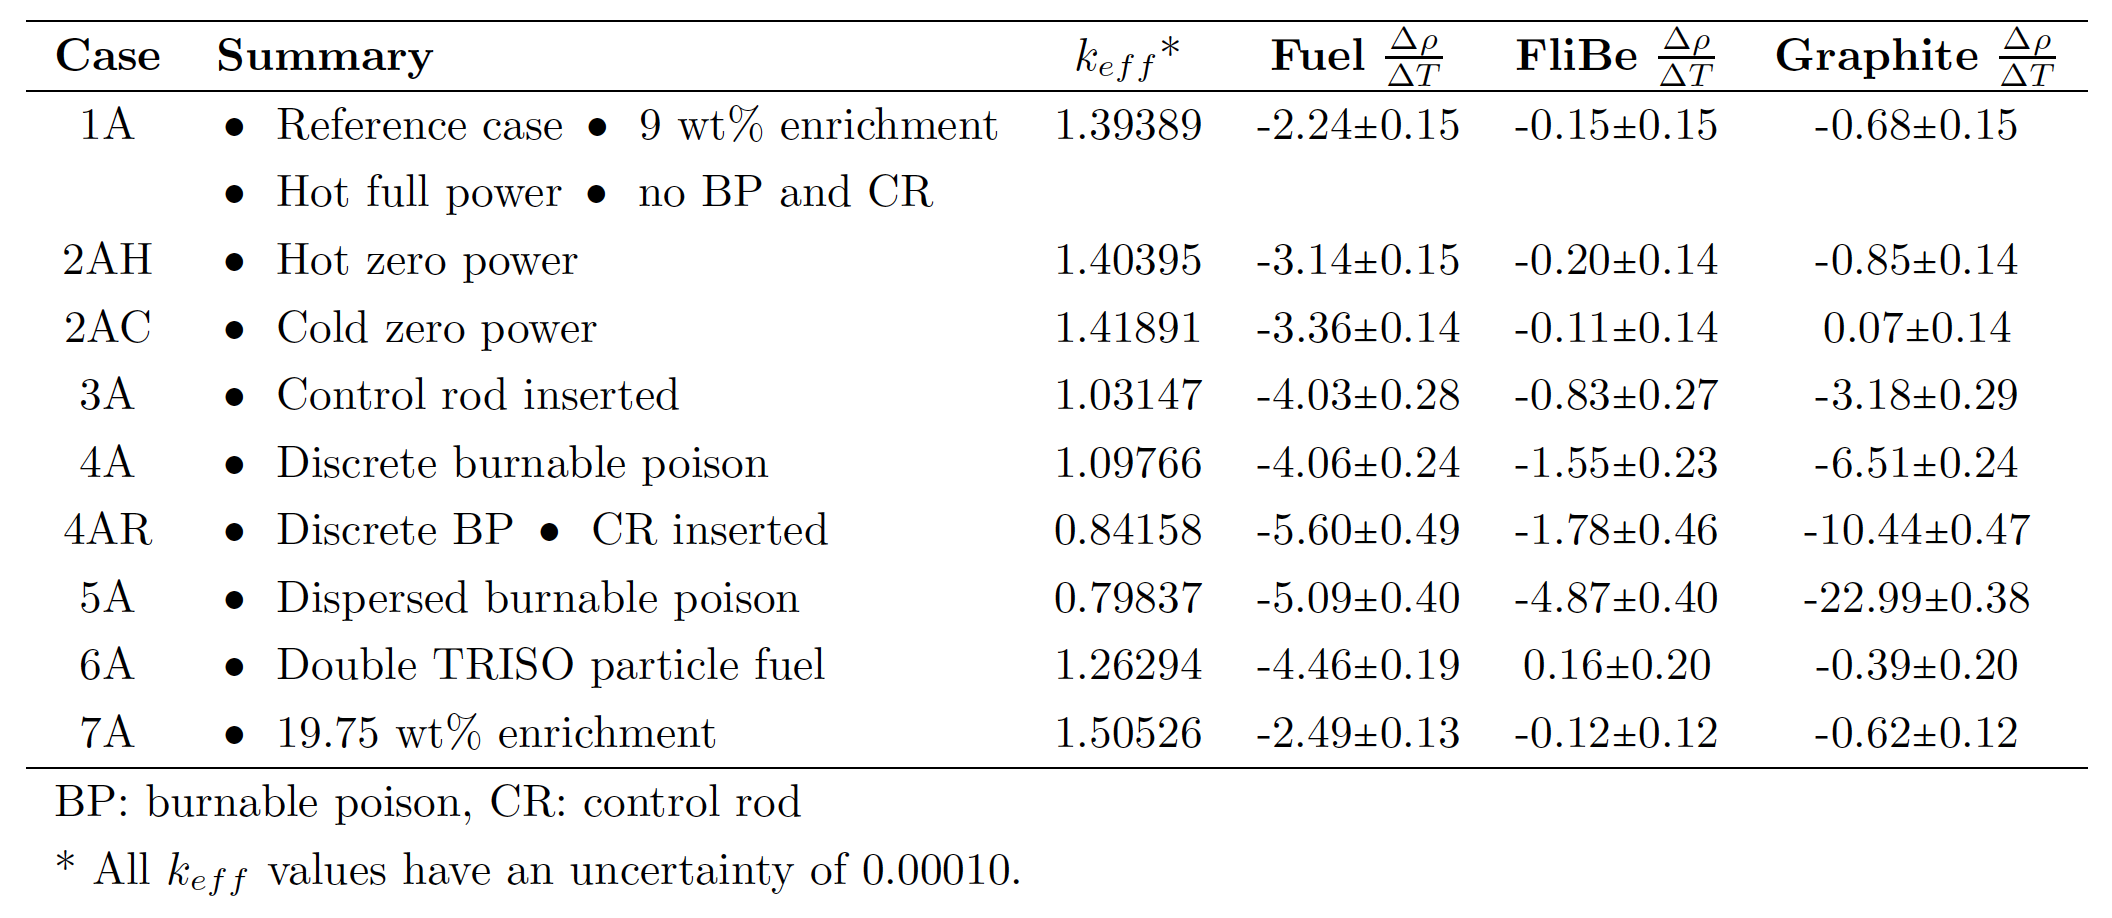
\includegraphics[width=\linewidth]{figures/benchmark-coeff-results.png}}
        \only<2>{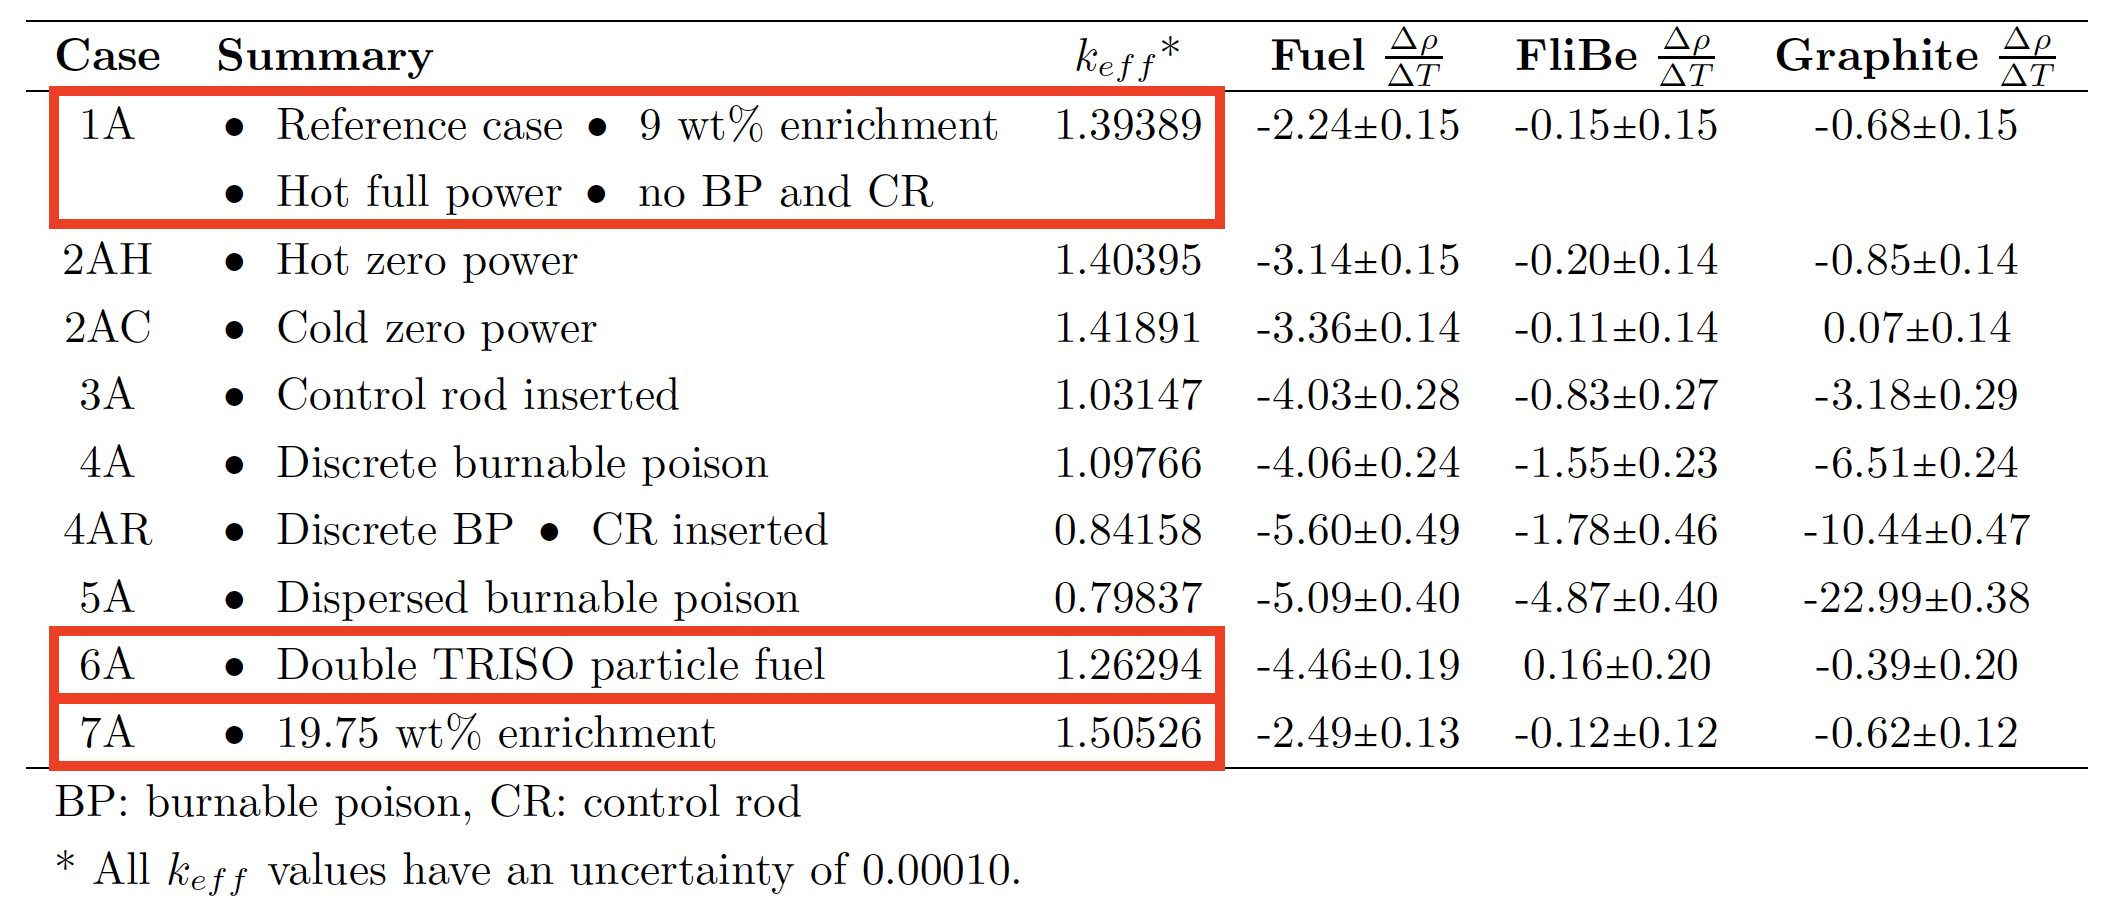
\includegraphics[width=\linewidth]{figures/benchmark-coeff-results-annotated.png}} 
    \end{table}
    500 active cycles, 100 inactive cycles, and 200000 neutrons
    UIUC's BlueWaters supercomputer with 64 XE nodes
\end{frame}

\begin{frame}
    \frametitle{FHR Benchmark Phase I-A Results}
    In an ANS M$\&$C 2021 conference paper we compared FHR benchmark participants' 
    Phase I-A $k_{eff}$ results. 
    \begin{figure}[]
        \centering
        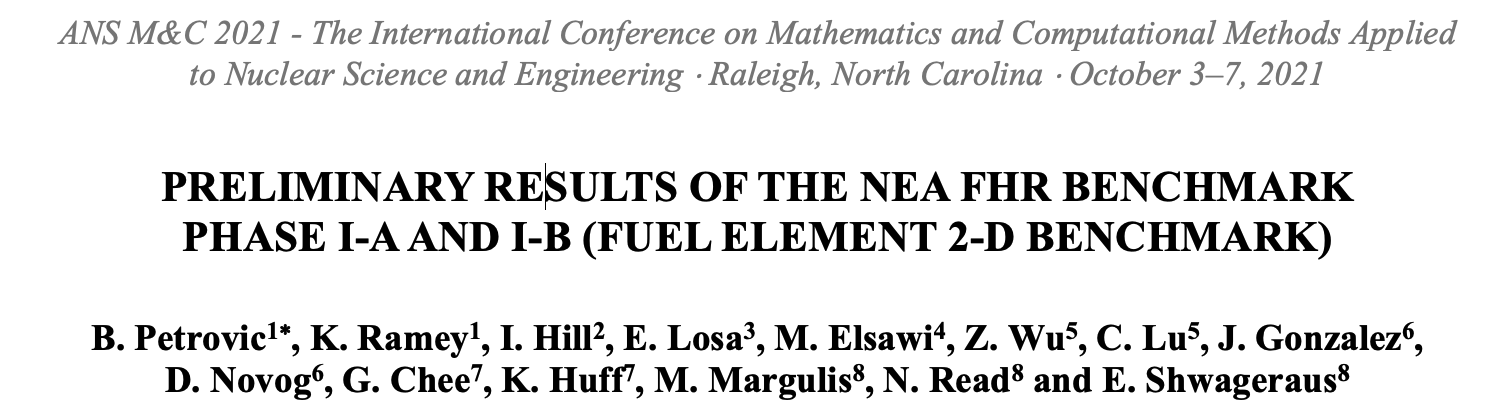
\includegraphics[width=0.85\linewidth]{figures/mnc.png} 
        \caption{FHR benchmark paper presented at M$\&$C 2021 
        \cite{petrovic_preliminary_2021}.}
    \end{figure}

    The standard deviation between participants for each case was in the 231 to 514 
    pcm range, \textbf{acceptable and notably close} given a blind benchmark.

    I am confident of an accurate AHTR base model. 
\end{frame}

\begin{frame}
    \frametitle{FHR Benchmark Phase I-A Results}
    \begin{figure}
        \centering
        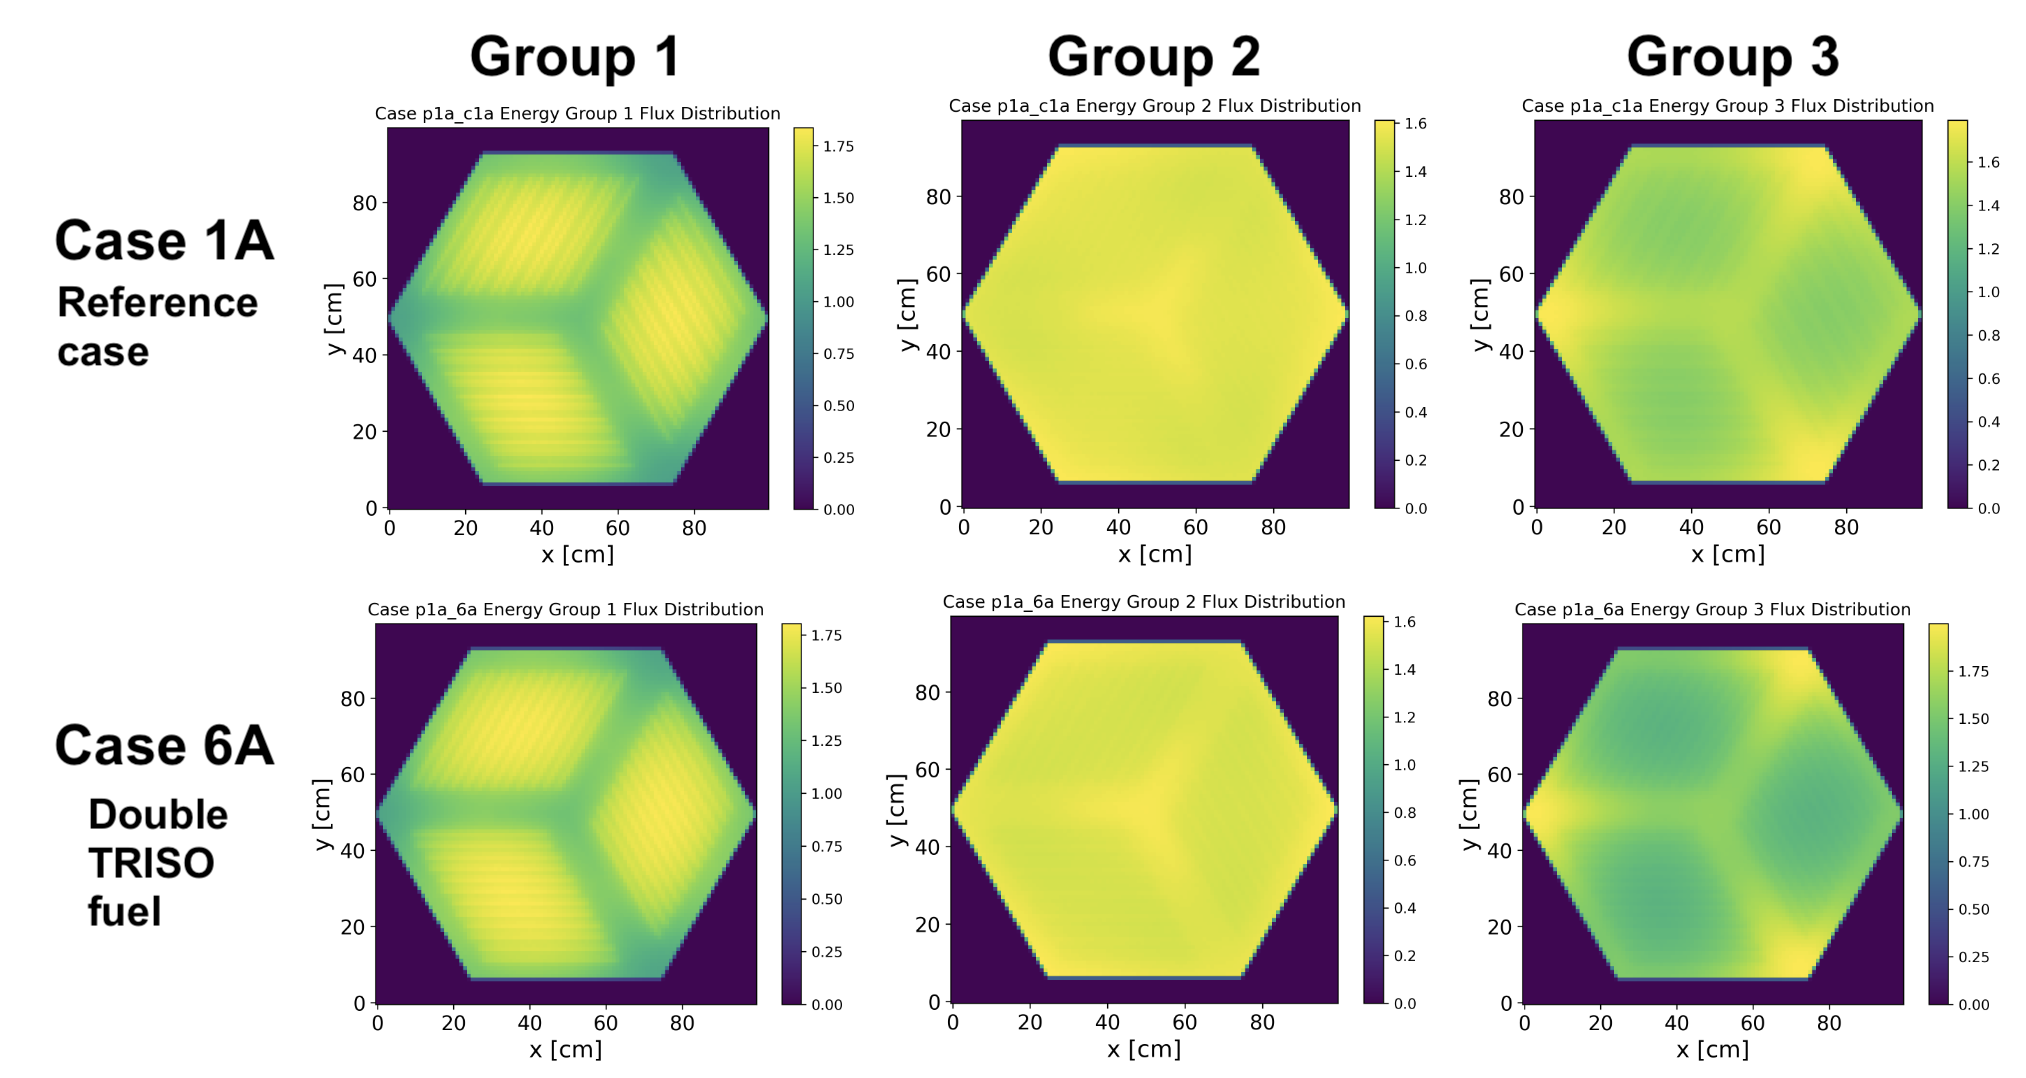
\includegraphics[width=\linewidth]{figures/phase1a-flux.png} 
        \vspace{-0.5cm}
        \caption{FHR Benchmark neutron flux distribution}
    \end{figure}
    \vspace{-0.3cm}
    \textbf{Increased fuel packing does not always correspond with increased keff 
    due to self-shielding effects.}
\end{frame}
